\chapter{Introduction}
\pagenumbering{arabic} 
\setcounter{page}{1} 

%Doing the biological experiments is programming
% The cell-free system is programmable matter, performing computation

% Use the autoencoder as a 

% General biological modeling
Despite more than a century of active biology research, running biological experiments is still time consuming and difficult.
Therefore, having a good computational model of the biological system of interest is incredibly valuable.
What makes a computational model good?
First of all, and most importantly, a good model needs to accurately describe how the biological system acts in the real world.
If the model accurately represents the biological system, then experiments can be run in silico instead of in vivo, speeding up the pace of research.
Secondly, a good model should be consistent--meaning its results vary only due to intrinsic biological sources of variation.
Though biological experiments can have wide variance due to external conditions, we want our model to vary due to the underlying biology.
Exact reproducibility is very difficult in laboratory environments, but a computer model can and should eliminate the extrinsic sources of variance that one encounters in a laboratory setting.
Finally, the best models not only describe the system, but also facilitate deeper insights into the underlying biology.
A good model should help researchers improve their understanding of the system that is modeled and provide a starting point for novel insights.

%Recent efforts to model biological systems have become ever more accurate as the amount of biological data collected increases.
Biological systems are incredibly complex and can be modeled at many different levels.
For example, there has been a recent rise in using multi-omic data--data that includes genomic, transcriptomic, metabolomic measurements--to model the behavior of an organism.
This dissertation will focus on using metabolic information to build a good computational model for a specific type of biological system called a cell-free system.
In particular, we use a variational autoencoder (VAE) on top of a metabolic model to determine which reactions are most important for cell-free systems.
The goal is to provide a model for biologists to better understand cell-free systems.
This will allow them to anticipate how different starting conditions will affect their experiments before actually running the experiment.

\textbf{Metabolic Models}
Metabolism involves all of the chemical reactions that occur within an organism in order to sustain its life and growth.
A huge number of applications in biology require examining the metabolism of an organism.
In particular, metabolic engineering has the potential to create advances in medicine and energy \cite{keasling2012synthetic}.
Thus, metabolic models have gained popularity over the past few decades as an important tool to understanding what is going on inside of a cell.
These models are used to predict how the phenotype of the organism will respond to various environmental inputs.

Most metabolic models involve mathematical representations of the processes occurring within the cell.
The different types of metabolic models are usually collected under the heading of constraint-based reconstruction and analysis (COBRA) models \cite{schellenberger2011quantitative}.
In particular, Flux Balance Analysis (FBA), is one of the most popular metabolic modeling techniques and has been used in applications from optimizing metabolic pathways \cite{almaas2004global} to investigating gene networks \cite{shlomi2007genome}.
FBA is applied to genome scale metabolic models (GEMs) to solve for a specific outcome of interest.
As progress has been made in the sequencing and understanding of the genomes of various organisms, these GEMs have become commonplace for many organisms.
However, these GEMs describe living organisms, not cell-free systems.

\textbf{Cell-Free Systems}
Cell free protein systems (CFPS) are a simplified version of cells that expose the crucial internal transcription and translation machinery, allowing the system to continue produce proteins without being alive.
The Central Dogma of biology is that "DNA makes RNA makes protein" \cite{}.
Cell-Free systems take that to an extreme by removing all endogenous DNA and RNA and membranes while retaining the proteins crucial for transcription and translation.
One can think of a CFPS as a type of programmable matter, similar to a biological computer.
They are computers because they "execute" any DNA "program" that is added to the mixture.
This means that when a DNA program is added to a cell-free system, the only protein that is being expressed is whatever is coded for in the custom protein.

CFPS are ideal in two respects for this dissertation.
First of all, running experiments in CFPS is much faster than typical in vivo methods because there is no need to grow cells.
Due to the time limitations of the dissertation schedule, this meant that we were able to generate relevant data within a few months instead of the years that a cell-based system could take.
Additionally, CFPS contain a strict subset of the reactions that occur in a cell-based system.
Therefore, we hypothesized that it would be easier to model a CFPS than a full E. coli system.

There have been a few attempts to model cell-free systems, which are explored in Section \ref{rw:mod-cf}.
However, very few of them have used metabolic models to examine cell-free systems.
Since CFPS are not living organisms, their functionality is entirely based on energy constraints.
So, it makes sense to examine these systems from the perspective of metabolism.
Existing metabolic models for CFPS are hand-constructed instead of using the GEMs that already exist for the original organism.
%The goal of this dissertation is to use machine learning in concert with already created FBA models to fit a metabolic model to these CFPS systems.

%\section{ML + Metabolic Models}

\textbf{Contributions}
This dissertation focuses on a number of novel aspects with regards to metabolic modeling and cell-free systems.
\begin{itemize}
\item This dissertation provides an automated reduction system that tailors GEMs specifically for cell-free systems.
That means the system can be used for any cell-free system which is derived from an organism that has a fully specified GEM, of which there are many dozens.
\item Additionally, it is the first use to our knowledge of applying deep learning or autoencoders to FBA models.
While PCA has been applied in the past, it lacks the generalizability of an autoencoder.
\item Finally, this dissertation provides an end-to-end system to accelerate the design-build-test (DBT) cycle of a lab.
Given biological data on one end, the computational pipeline then produces a model that allows the prediction of data for subsequent experiments.
\end{itemize}
%VAE
%experiments + computational
%latent representation

\textbf{Paper outline}
The structure of this dissertation is as follows.
The next chapter provides background and related work.
We focus on describing the current state of the art in metabolic modeling, specifically focusing on FBA and the creation of a GEM for E. coli.
Next, we focus on efforts to model cell-free systems, describing the few examples of FBA applied to cell-free systems.
Then, we describe the relevant literature in autoencoders, in particular VAEs.
Finally, we describe previous applications of machine learning to FBA.

\begin{figure}[t!]
\begin{center}
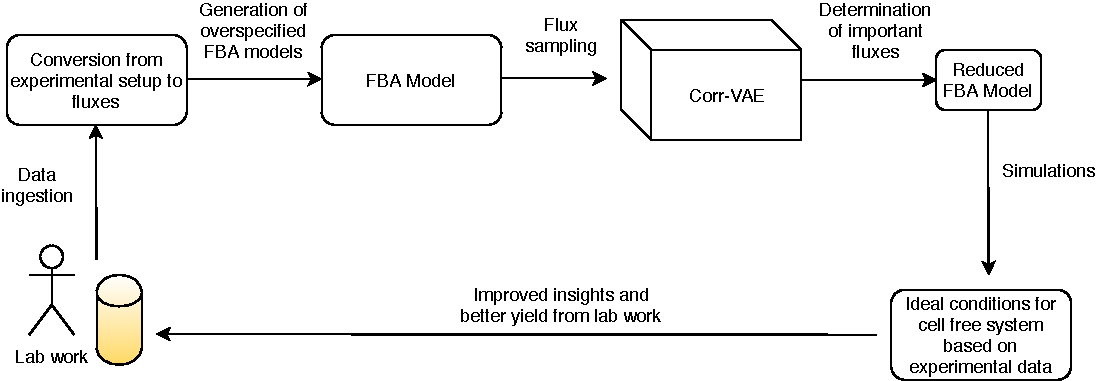
\includegraphics[width=\textwidth]{figs/SystemOverview.pdf}
\end{center}
\label{fig:overview}
\caption{A figure showing the overall pipeline for the system to generate cell-free metabolic models.}
\end{figure}

Chapter \ref{chap:impl} describes the system we have designed and built to model cell-free systems.
The entire pipeline is shown in fig \ref{fig:overview}.
We begin by describing the biological experiments and the type of data that was generated.
Next, we describe how to ingest the experimental setup and convert it into various FBA models.
Then, we explain how we flux sampled from the FBA models to generate a larger dataset for our deep learning algorithms.
That dataset is then ran through a VAE, which generates a latent representation.
That latent representation is used to reduce the FBA models.
Finally, we describe how we the reduced FBA model to improve future experimental yield.

Chapter \ref{chap:res} describes the results of the experiments.
This includes results showing the improvment of my technique over naive solutions as well as novel biological insights that were unearthed due to my system.

Finally, we conclude with a chapter of discussion and directions of future work in this area.
